\documentclass[aspectratio=169, 10pt]{beamer}

% --- THEME & STYLING ---
\usetheme{Madrid}
\usefonttheme{professionalfonts}

% --- ESSENTIAL PACKAGES ---
\usepackage[utf8]{inputenc}
\usepackage[english]{babel}
\usepackage{amsmath, amssymb, amsfonts}
\usepackage{graphicx}
\usepackage{booktabs}
\usepackage{array}
\usepackage{hyperref}

% --- COLOR DEFINITIONS ---
\definecolor{primaryNavy}{RGB}{20, 45, 85}
\definecolor{accentTeal}{RGB}{13, 148, 136}
\definecolor{accentOrange}{RGB}{217, 95, 2}
\definecolor{bgSlate}{RGB}{248, 250, 252}
\definecolor{textDark}{RGB}{30, 41, 59}

\setbeamercolor{palette primary}{bg=primaryNavy, fg=white}
\setbeamercolor{palette secondary}{bg=accentTeal, fg=white}
\setbeamercolor{palette tertiary}{bg=primaryNavy!90, fg=white}
\setbeamercolor{title}{bg=primaryNavy, fg=white}
\setbeamercolor{frametitle}{bg=primaryNavy, fg=white}
\setbeamercolor{structure}{fg=primaryNavy}
\setbeamercolor{block title}{bg=primaryNavy, fg=white}
\setbeamercolor{block body}{bg=primaryNavy!8, fg=textDark}
\setbeamercolor{block title alerted}{bg=accentOrange, fg=white}
\setbeamercolor{block body alerted}{bg=accentOrange!10, fg=textDark}
\setbeamercolor{block title example}{bg=accentTeal, fg=white}
\setbeamercolor{block body example}{bg=accentTeal!10, fg=textDark}

% Remove navigation symbols
\setbeamertemplate{navigation symbols}{}

% Custom footer
\setbeamertemplate{footline}{
  \leavevmode%
  \hbox{%
  \begin{beamercolorbox}[wd=.333333\paperwidth,ht=2.25ex,dp=1ex,center]{author in head/foot}%
    \usebeamerfont{author in head/foot}Kien Nguyen \quad (\texttt{kien3007})
  \end{beamercolorbox}%
  \begin{beamercolorbox}[wd=.333333\paperwidth,ht=2.25ex,dp=1ex,center]{title in head/foot}%
    \usebeamerfont{title in head/foot}Household Purchase Propensity Model
  \end{beamercolorbox}%
  \begin{beamercolorbox}[wd=.333333\paperwidth,ht=2.25ex,dp=1ex,right]{date in head/foot}%
    \usebeamerfont{date in head/foot}\insertframenumber{} / \inserttotalframenumber\hspace*{2ex}
  \end{beamercolorbox}}%
  \vskip0pt%
}

% --- METADATA ---
\title[Purchase Propensity Modeling]{\textbf{Household Purchasing Propensity Modeling}}
\subtitle{A Rigorous Point-in-Time Machine Learning Framework on 2.6M Dunnhumby Transactions}
\author{\textbf{Kien Nguyen}}
\institute[Data Science \& Retail AI]{
  Faculty of Computer Science \& Data Science\\
  \texttt{https://github.com/kien3007/purchasing-propensity-model}
}
\date{November 2026}

\begin{document}

% ==============================================================================
% SLIDE 1: TITLE SLIDE
% ==============================================================================
\begin{frame}[plain]
  \titlepage
\end{frame}

% ==============================================================================
% SLIDE 2: EXECUTIVE SUMMARY & RESEARCH MOTIVATION
% ==============================================================================
\begin{frame}{1. Executive Motivation \& Problem Statement}
  \begin{columns}[T]
    \begin{column}{0.55\textwidth}
      \textbf{Core Retail Challenge:}
      \begin{itemize}
        \item Supermarket chains face tight margins and high promotional costs.
        \item Blasting discounts indiscriminately wastes budget on customers who would buy anyway (\textit{Organic/Sure Things}).
        \item Traditional propensity models often suffer from \textbf{future data leakage} and uncalibrated probabilities.
      \end{itemize}
      \vspace{0.3cm}
      \begin{alertblock}{Research Objective}
        Predict whether household $h \in \{1 \dots 2500\}$ will generate \textbf{at least one valid basket} ($> \$0$) in future window $\Delta t = 14$ days, using strictly historical data ($DAY \le t_0$).
      \end{alertblock}
    \end{column}
    
    \begin{column}{0.42\textwidth}
      \begin{block}{Project Hallmarks}
        \begin{itemize}
          \item \textbf{100\% Real Data:} 2,595,732 transaction records from Dunnhumby.
          \item \textbf{Zero Future Leakage:} Multi-cutoff Point-in-Time temporal barriers.
          \item \textbf{Calibrated Confidence:} Isotonic regression ensures $P(Y=1)$ reflects true business frequency.
          \item \textbf{Reproducibility:} Modular package, 4 unit tests passing, full documentation.
        \end{itemize}
      \end{block}
    \end{column}
  \end{columns}
\end{frame}

% ==============================================================================
% SLIDE 3: MATHEMATICAL FORMULATION
% ==============================================================================
\begin{frame}{2. Mathematical Formulation \& Point-in-Time Discipline}
  \begin{block}{Definition of Target Variable ($Y_{h, t_0}$)}
    For an arbitrary temporal cutoff date $t_0$, observation lookback $W_{obs} = 180$ days, and prediction horizon $\Delta t = 14$ days:
    \[
      Y_{h, t_0} = \begin{cases}
        1 & \text{if } \exists \text{ valid basket of household } h \text{ in } (t_0, t_0 + \Delta t] \\
        0 & \text{otherwise}
      \end{cases}
    \]
  \end{block}
  \vspace{0.2cm}
  \begin{columns}[T]
    \begin{column}{0.50\textwidth}
      \textbf{Temporal Sliding Windows:}
      \begin{itemize}
        \item \textbf{Historical Window:} $[t_0 - W_{obs}, t_0]$ (Strictly past data).
        \item \textbf{Target Window:} $(t_0, t_0 + \Delta t]$ (Strictly future ground truth).
        \item \textbf{Zero Contamination:} Features computed at $t_0$ have zero access to $DAY > t_0$.
      \end{itemize}
    \end{column}
    \begin{column}{0.48\textwidth}
      \begin{exampleblock}{Multi-Cutoff Sliding Sampling}
        To maximize sample efficiency without temporal leakage:
        \begin{itemize}
          \item \textbf{Train:} 11 cutoffs $t_0 \in [200, 500]$ ($N = 27,500$)
          \item \textbf{Val:} 3 cutoffs $t_0 \in [530, 590]$ ($N = 7,500$)
          \item \textbf{Test (OOT):} 2 cutoffs $t_0 \in [650, 680]$ ($N = 5,000$)
        \end{itemize}
      \end{exampleblock}
    \end{column}
  \end{columns}
\end{frame}

% ==============================================================================
% SLIDE 4: RELATIONAL DATA ARCHITECTURE
% ==============================================================================
\begin{frame}{3. Relational Data Architecture \& Cleansing Audit}
  \begin{table}[h]
    \centering
    \small
    \begin{tabular}{llrrl}
      \toprule
      \textbf{Table Name} & \textbf{Primary Key} & \textbf{Rows} & \textbf{Coverage} & \textbf{Role in Propensity Framework} \\
      \midrule
      \texttt{transaction\_data} & Receipt Line Item & 2,595,732 & 2,500 HH & Raw transactions (Day 1 to 711) \\
      \texttt{product} & \texttt{PRODUCT\_ID} & 92,353 & 44 Depts & Department \& fresh food identification \\
      \texttt{hh\_demographic} & \texttt{household\_key} & 801 & 32.0\% & Socioeconomic \& family size context \\
      \texttt{campaign\_desc} & \texttt{CAMPAIGN} & 30 & Full & Marketing campaign temporal schedule \\
      \texttt{campaign\_table} & \texttt{CAMPAIGN + HH} & 7,208 & 1,584 HH & Direct-to-household target assignment \\
      \texttt{coupon} & \texttt{COUPON\_UPC} & 124,548 & Full & Coupon-to-product SKU mappings \\
      \texttt{coupon\_redempt} & Redemption Event & 2,318 & 434 HH & Historical coupon redemption logs \\
      \bottomrule
    \end{tabular}
  \end{table}
  \begin{alertblock}{Data Cleaning \& Normalization}
    \begin{itemize}
      \item Cleaned 942 void/refund transactions ($\text{Spend} \le \$0$) $\rightarrow$ \textbf{275,542 valid trip-level baskets}.
      \item Downcasted data types to 8/16/32-bit representations, reducing memory footprint by \textbf{78\%} (from 350MB to 70MB).
    \end{itemize}
  \end{alertblock}
\end{frame}

% ==============================================================================
% SLIDE 5: EMPIRICAL DISCOVERY 1 - THE SHOPPING CADENCE
% ==============================================================================
\begin{frame}{4. Empirical Discovery: The Natural Shopping Cadence}
  \begin{columns}[c]
    \begin{column}{0.55\textwidth}
      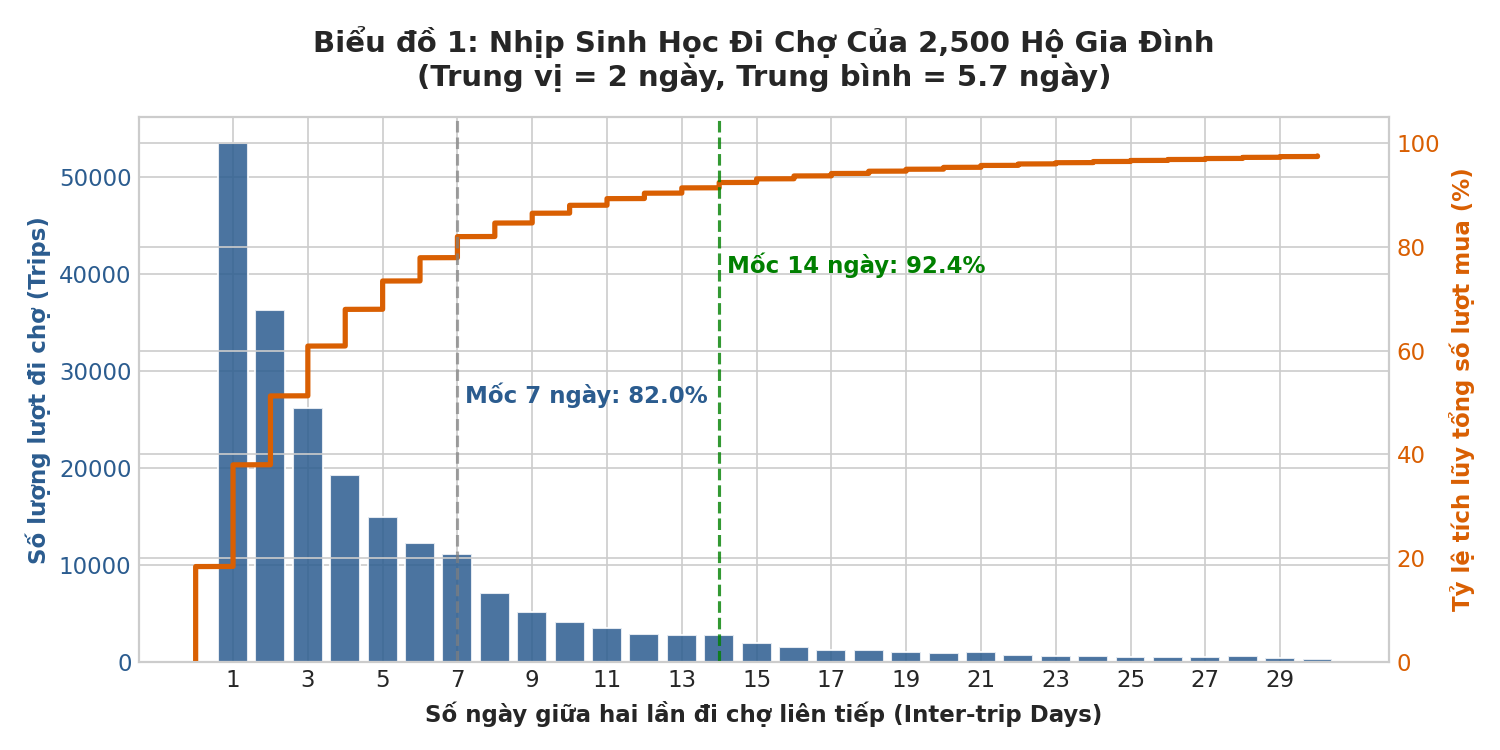
\includegraphics[width=\textwidth]{../reports/figures/01_inter_trip_distribution.png}
    \end{column}
    \begin{column}{0.42\textwidth}
      \textbf{Inter-trip Days ($\Delta \text{DAY}$):}
      \begin{itemize}
        \item \textbf{Median Gap:} \textbf{2.0 days}
        \item \textbf{Mean Gap:} \textbf{5.67 days}
        \item \textbf{P75 / P90:} 6.0 days / 12.0 days
      \end{itemize}
      \vspace{0.2cm}
      \begin{block}{Scientific Validation for $\Delta t = 14$}
        \begin{itemize}
          \item $\le 7$ days: \textbf{82.0\%} of all trips
          \item $\le 14$ days: \textbf{92.4\%} of all trips
          \item $\le 30$ days: \textbf{97.5\%} of all trips
        \end{itemize}
        Setting $\Delta t = 14$ days captures the full replenishment cycle while preserving actionable lead time.
      \end{block}
    \end{column}
  \end{columns}
\end{frame}

% ==============================================================================
% SLIDE 6: EMPIRICAL DISCOVERY 2 - BASKET SPEND ANATOMY
% ==============================================================================
\begin{frame}{5. Empirical Discovery: Basket Value \& Spending Power}
  \begin{columns}[c]
    \begin{column}{0.55\textwidth}
      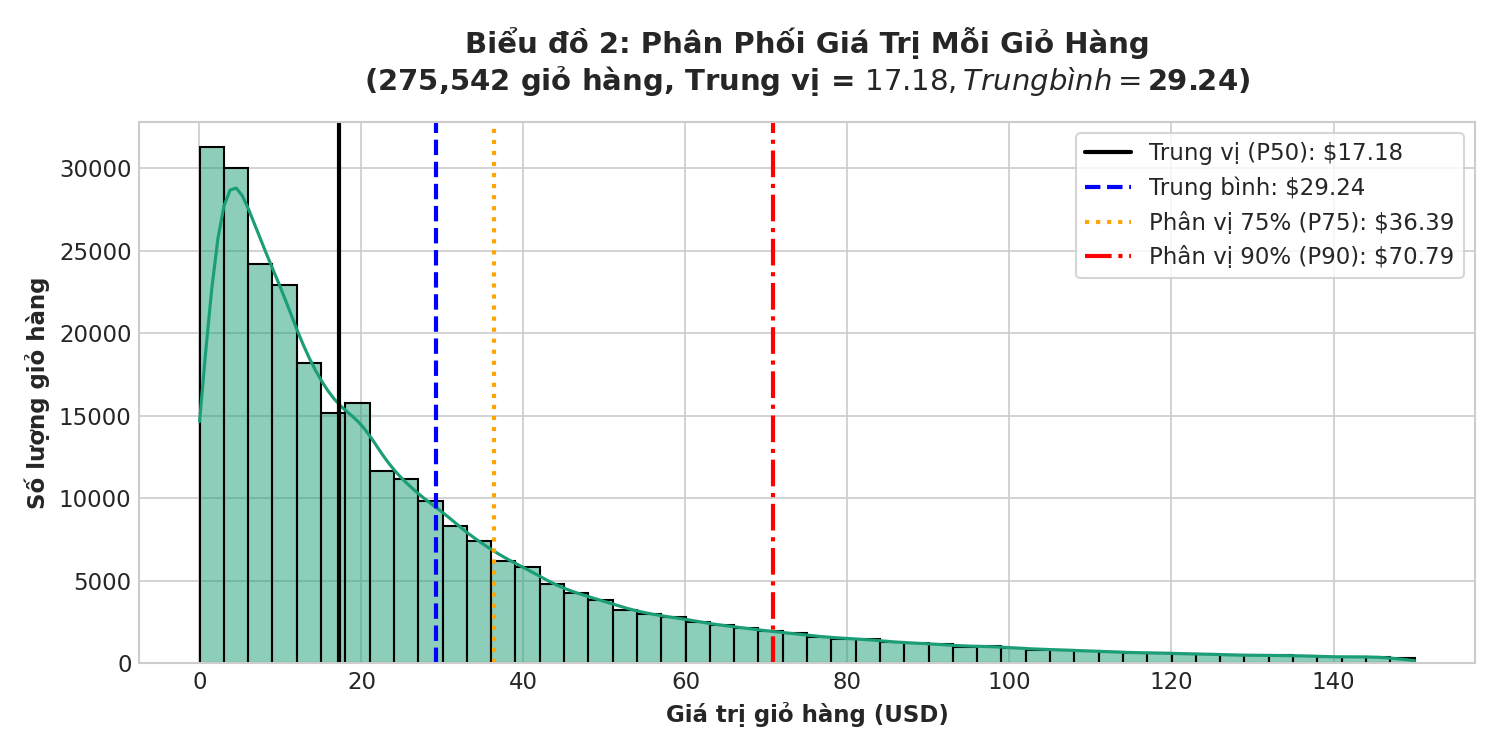
\includegraphics[width=\textwidth]{../reports/figures/02_basket_spend_distribution.png}
    \end{column}
    \begin{column}{0.42\textwidth}
      \textbf{Basket Spend Statistics ($N = 275,542$):}
      \begin{itemize}
        \item \textbf{Median (P50):} \textbf{\$17.18}
        \item \textbf{Mean (AOV):} \textbf{\$29.24}
        \item \textbf{P75 / P90:} \$37.28 / \$68.04
      \end{itemize}
      \vspace{0.2cm}
      \begin{exampleblock}{Feature Engineering Takeaway}
        Strong right-skewed distribution.
        \begin{itemize}
          \item Quick-fill trips dominate count ($\le \$20$).
          \item Major stock-up trips dominate revenue ($> \$60$).
          \item Model must decouple \textbf{Trip Frequency} from \textbf{Monetary AOV}.
        \end{itemize}
      \end{exampleblock}
    \end{column}
  \end{columns}
\end{frame}

% ==============================================================================
% SLIDE 7: EMPIRICAL DISCOVERY 3 - FRESH FOOD & TIMING
% ==============================================================================
\begin{frame}{6. Behavioral Triggers: Perishables \& Daily Rhythm}
  \begin{columns}[c]
    \begin{column}{0.48\textwidth}
      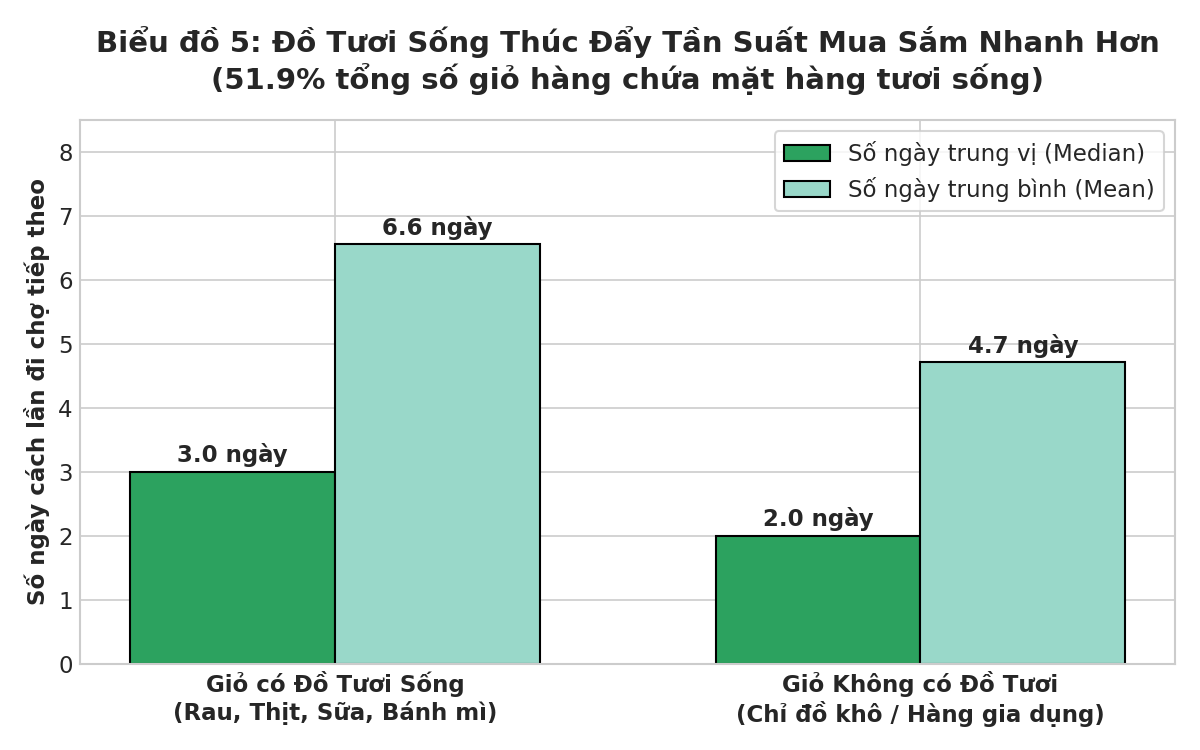
\includegraphics[width=\textwidth]{../reports/figures/05_perishable_trigger_effect.png}
      \centering
      \small \textbf{Figure 5:} Perishable Fresh Food Acceleration
    \end{column}
    \begin{column}{0.48\textwidth}
      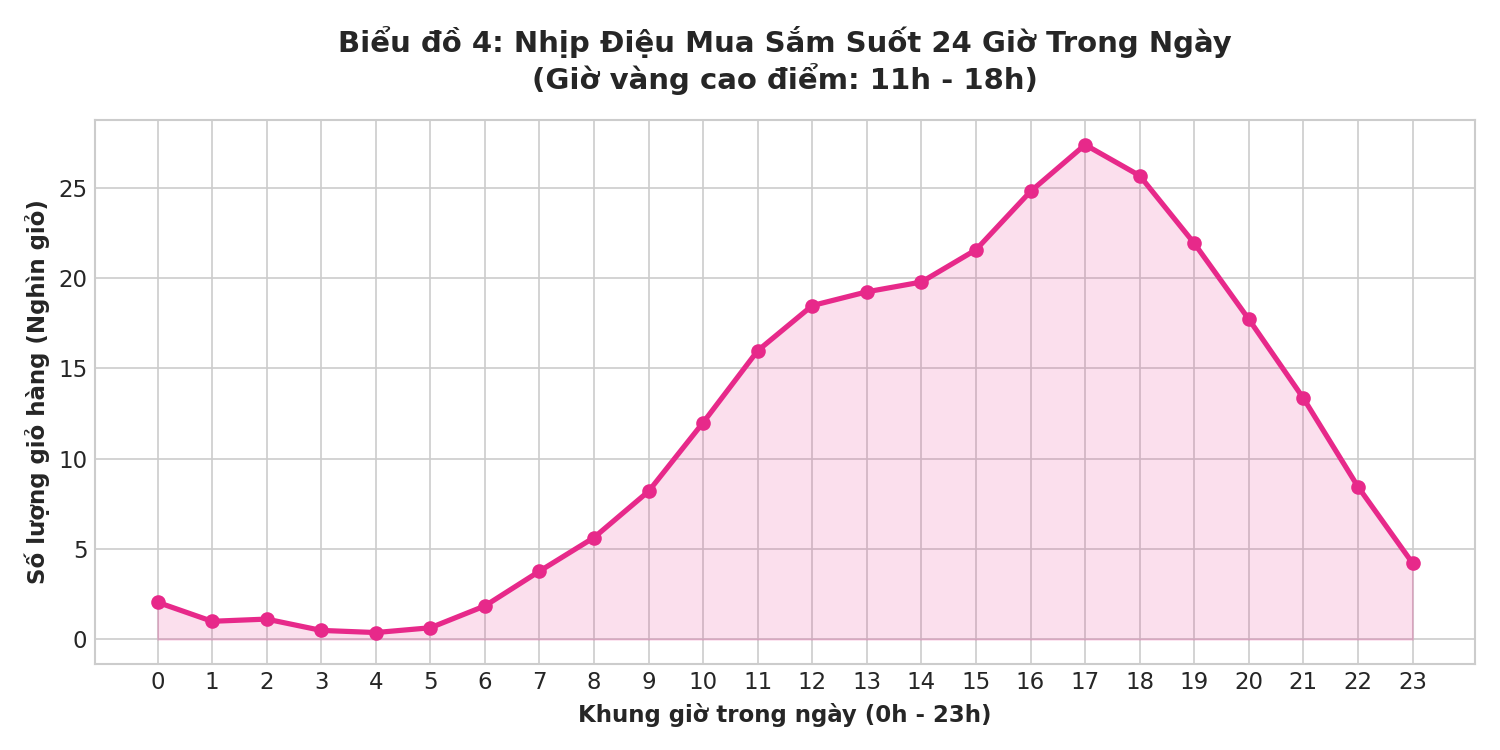
\includegraphics[width=\textwidth]{../reports/figures/04_hourly_shopping_rhythm.png}
      \centering
      \small \textbf{Figure 4:} 24-Hour Intraday Shopping Rhythm
    \end{column}
  \end{columns}
  \vspace{0.2cm}
  \begin{itemize}
    \item \textbf{Perishable Food Trigger:} \textbf{51.71\%} of baskets contain fresh goods (Produce, Meat, Dairy, Bakery). Perishable inventory decays rapidly $\rightarrow$ creates urgent replenishment trips.
    \item \textbf{Shopping Hours:} Peak volume concentrated between \textbf{11:00 and 18:00} ($>65\%$ of daily transactions).
  \end{itemize}
\end{frame}

% ==============================================================================
% SLIDE 8: EMPIRICAL DISCOVERY 4 - COUPON & MARKETING ACCELERATION
% ==============================================================================
\begin{frame}{7. Marketing Responsiveness: Coupon Halo \& Campaigns}
  \begin{columns}[c]
    \begin{column}{0.54\textwidth}
      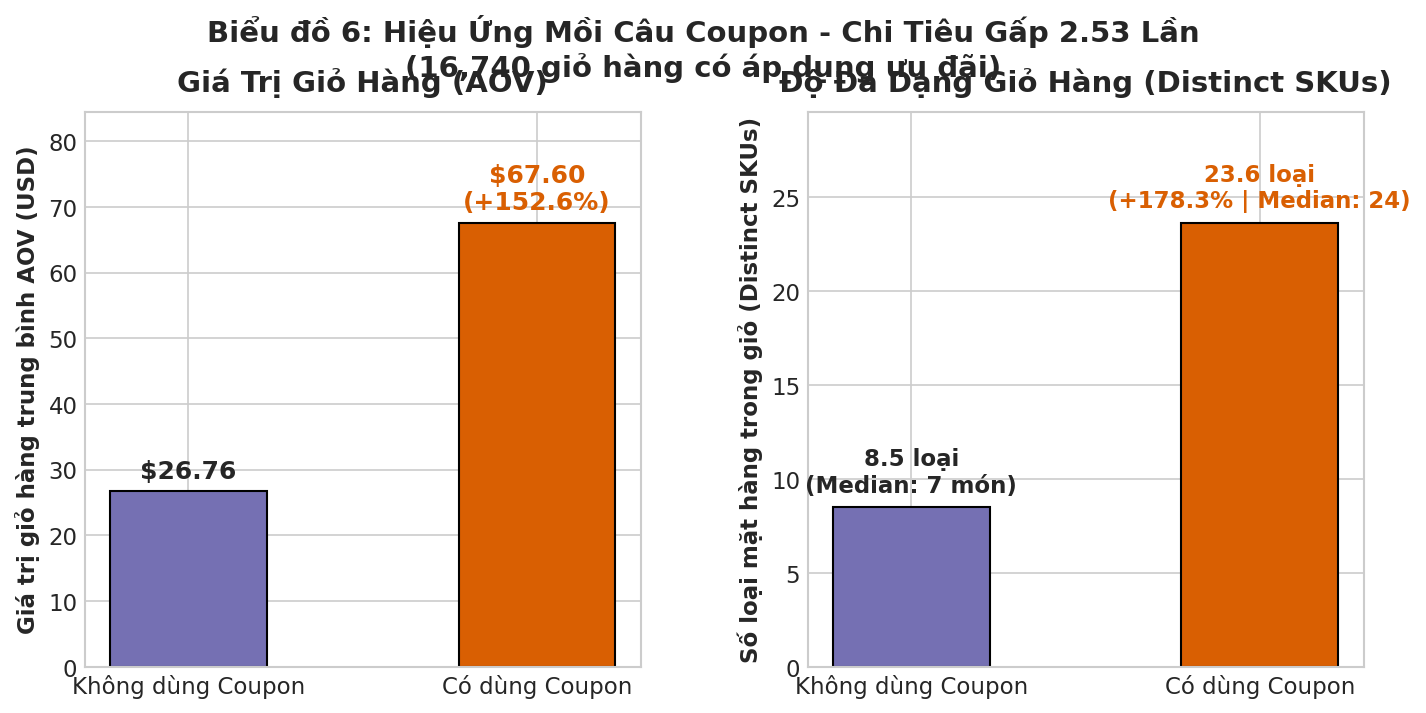
\includegraphics[width=\textwidth]{../reports/figures/06_coupon_halo_effect.png}
      \centering
      \small \textbf{Figure 6:} Coupon Halo Spend \& Breadth Lift
    \end{column}
    \begin{column}{0.44\textwidth}
      \begin{block}{The Coupon Halo Effect}
        \begin{itemize}
          \item AOV with Coupon: \textbf{\$67.60} vs without: \textbf{\$26.76} (\textbf{+152.6\% / 2.53x}).
          \item Distinct SKUs: \textbf{23.6} vs \textbf{8.5} (\textbf{+178.3\% / 2.78x}).
          \item Coupons trigger major basket expansion.
        \end{itemize}
      \end{block}
      \begin{exampleblock}{Campaign Trip Acceleration}
        \begin{itemize}
          \item In Active Campaign: \textbf{3.55 days} cadence.
          \item Outside Campaign: \textbf{6.49 days} cadence.
          \item \textbf{45.3\% reduction} in inter-trip interval!
        \end{itemize}
      \end{exampleblock}
    \end{column}
  \end{columns}
\end{frame}

% ==============================================================================
% SLIDE 9: EMPIRICAL DISCOVERY 5 - STORE LOYALTY & DEMOGRAPHICS
% ==============================================================================
\begin{frame}{8. Demographics \& Store Loyalty Dynamics}
  \begin{columns}[c]
    \begin{column}{0.48\textwidth}
      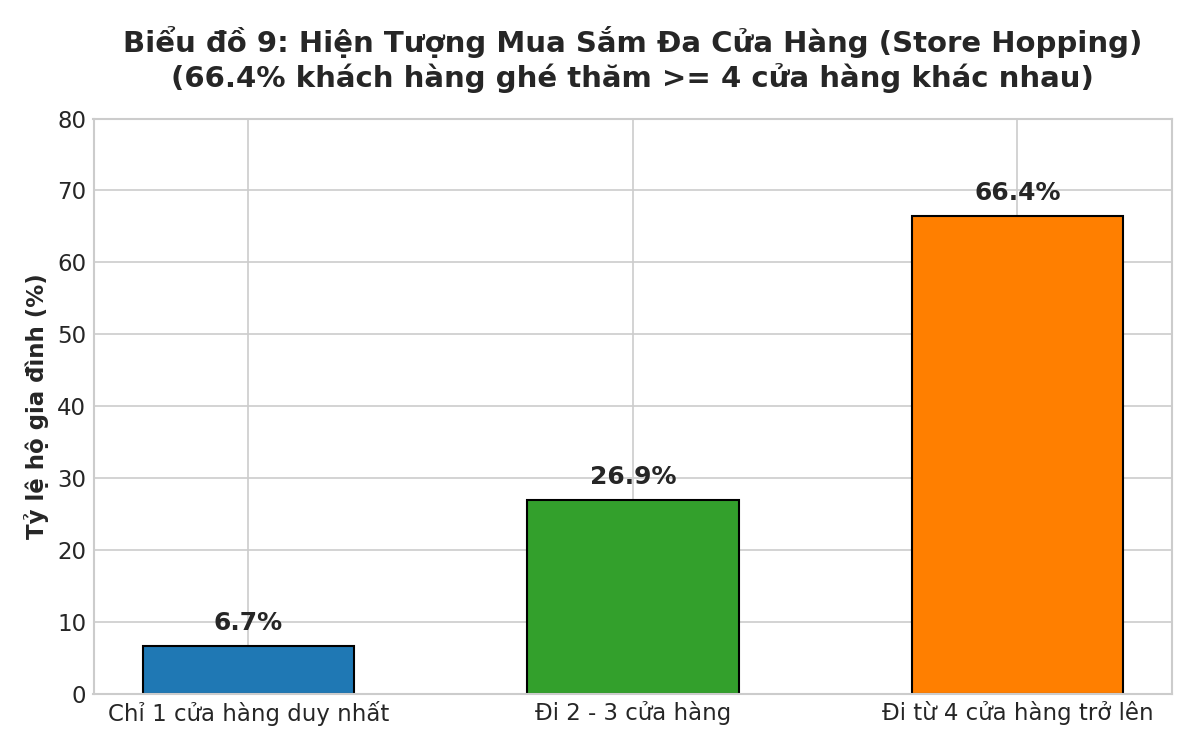
\includegraphics[width=\textwidth]{../reports/figures/08_store_hopping_distribution.png}
      \centering
      \small \textbf{Figure 8:} Store Hopping Behavior
    \end{column}
    \begin{column}{0.48\textwidth}
      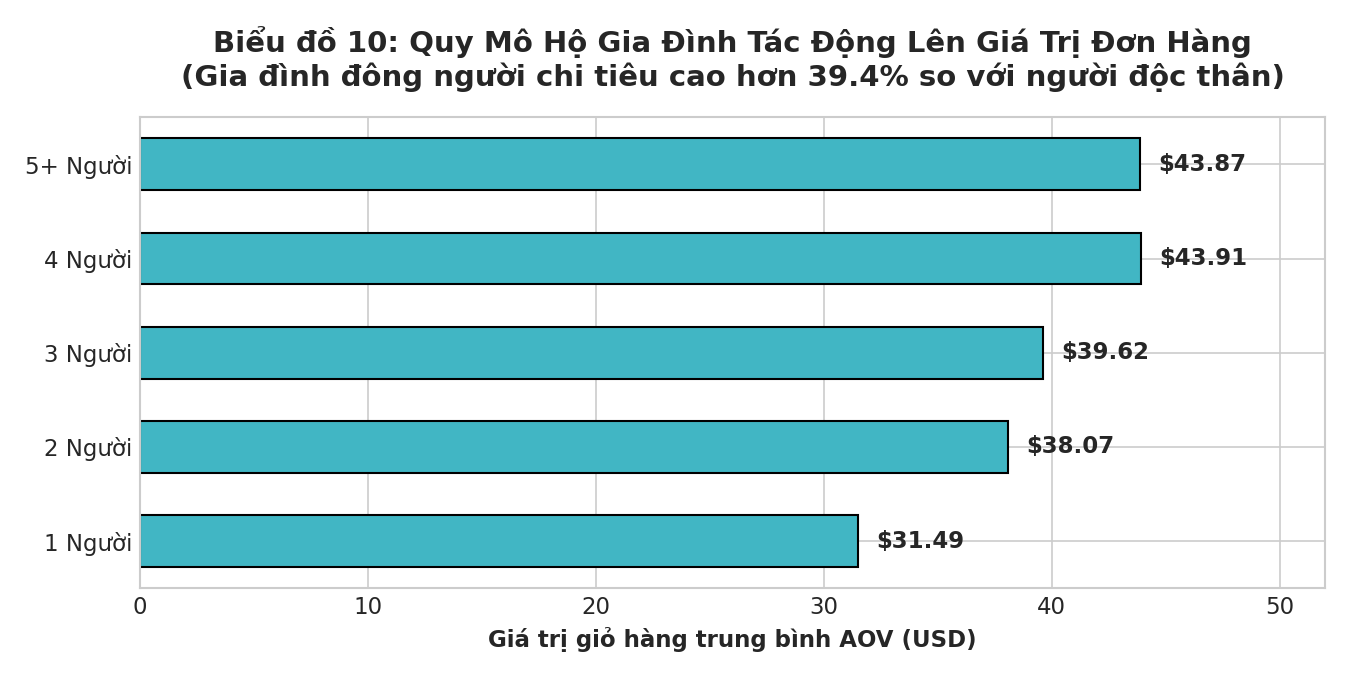
\includegraphics[width=\textwidth]{../reports/figures/09_household_size_vs_aov.png}
      \centering
      \small \textbf{Figure 9:} Household Size vs Basket AOV
    \end{column}
  \end{columns}
  \vspace{0.2cm}
  \begin{itemize}
    \item \textbf{Store Hopping:} Only 6.68\% visit 1 store; \textbf{66.4\% visit $\ge 4$ stores}. Yet, primary store captures \textbf{73.35\% of total household spend}.
    \item \textbf{Demographic Impact:} Large families (4-5+ members) spend \textbf{\$43.91} AOV vs \textbf{\$31.49} for single households (\textbf{+39.4\% spend expansion}).
  \end{itemize}
\end{frame}

% ==============================================================================
% SLIDE 10: POINT-IN-TIME FEATURE ENGINEERING
% ==============================================================================
\begin{frame}{9. Multi-Dimensional Feature Engineering (28 Features)}
  \begin{table}[h]
    \centering
    \footnotesize
    \begin{tabular}{lp{6.2cm}p{4.2cm}}
      \toprule
      \textbf{Dimension} & \textbf{Key Extracted Features} & \textbf{Business Justification} \\
      \midrule
      \textbf{Recency \& Cycle} & \texttt{days\_since\_last\_basket}, \texttt{median\_inter\_trip}, \texttt{std\_inter\_trip}, \texttt{urgency\_ratio} & Captures personal lateness ($Recency / Cadence$). \\
      \textbf{Perishable Velocity} & \texttt{days\_since\_last\_perishable}, \texttt{perishable\_basket\_ratio\_90d} & Measures biological urgency of fresh food depletion. \\
      \textbf{Frequency \& Momentum} & \texttt{baskets\_count\_14d/30d/60d/90d/180d}, \texttt{frequency\_momentum\_30\_vs\_90} & Distinguishes steady habit from recent velocity shifts. \\
      \textbf{Monetary \& Breadth} & \texttt{spend\_30d/90d/180d}, \texttt{aov\_90d}, \texttt{avg\_items\_per\_basket\_90d} & Quantifies household purchasing power. \\
      \textbf{Marketing \& Promotion} & \texttt{is\_targeted\_by\_active\_campaign}, \texttt{coupon\_redemption\_count\_180d} & Measures promotional pull and coupon responsiveness. \\
      \textbf{Store Loyalty} & \texttt{store\_loyalty\_index}, \texttt{primary\_store\_id} & Captures channel stickiness and geographic affinity. \\
      \textbf{Demographics} & \texttt{classification\_1} to \texttt{classification\_5}, \texttt{KID\_CATEGORY\_DESC} & Prior for cold-start and family size demand. \\
      \bottomrule
    \end{tabular}
  \end{table}
\end{frame}

% ==============================================================================
% SLIDE 11: TARGET STABILITY OVER TIME
% ==============================================================================
\begin{frame}{10. Target Label Stability Across Sliding Cutoffs}
  \begin{columns}[c]
    \begin{column}{0.55\textwidth}
      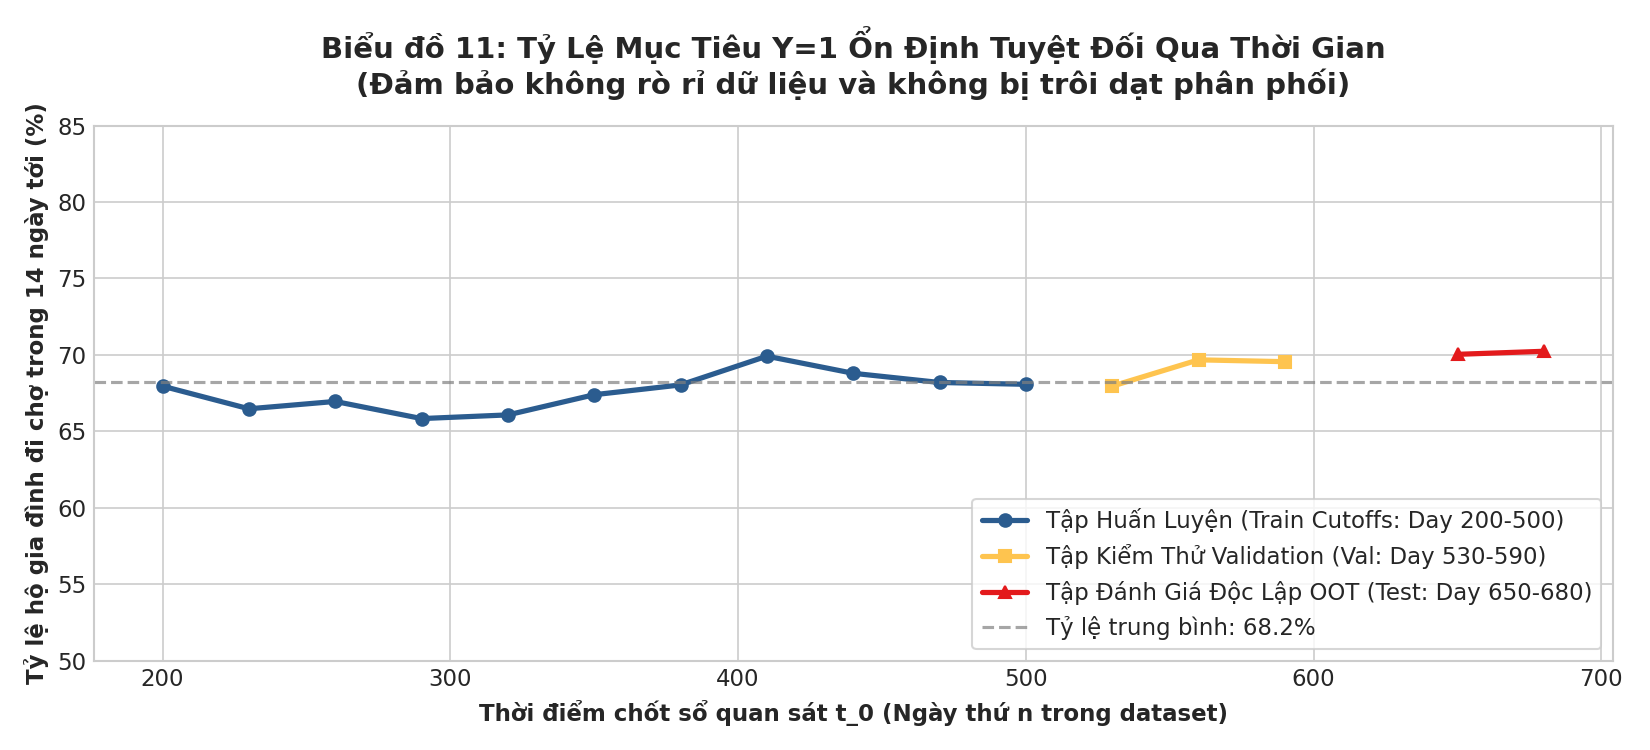
\includegraphics[width=\textwidth]{../reports/figures/10_target_rate_stability.png}
    \end{column}
    \begin{column}{0.42\textwidth}
      \textbf{Temporal Stationarity Audit:}
      \begin{itemize}
        \item 16 sliding cutoff points from Day 200 to Day 680 ($\sim 1.5$ years).
        \item \textbf{Mean Positive Rate:} \textbf{68.25\%}
        \item \textbf{Min / Max Rate:} 65.84\% / 70.24\%
      \end{itemize}
      \vspace{0.2cm}
      \begin{block}{Methodological Soundness}
        The target variable exhibits remarkable temporal stability (narrow $\pm 2.5\%$ band).
        Confirms no extreme concept drift or seasonal distortion across time splits.
      \end{block}
    \end{column}
  \end{columns}
\end{frame}

% ==============================================================================
% SLIDE 12: MODEL BENCHMARKING HIERARCHY
% ==============================================================================
\begin{frame}{11. Three-Tier Model Benchmarking Hierarchy}
  \begin{columns}[T]
    \begin{column}{0.32\textwidth}
      \begin{block}{\textbf{Tier 1: Retail Heuristic}}
        \textbf{Urgency Ratio Rule:}
        \[
          \hat{P}_h = \sigma\left(k \cdot \left(\frac{\text{Recency}}{\text{Cadence}} - 0.8\right)\right)
        \]
        \begin{itemize}
          \item Rule-of-thumb baseline.
          \item Predicts purely on individual lateness.
        \end{itemize}
      \end{block}
    \end{column}
    \begin{column}{0.32\textwidth}
      \begin{block}{\textbf{Tier 2: Logistic Regression}}
        \textbf{Linear Benchmark:}
        \begin{itemize}
          \item Median imputation.
          \item Robust Standard Scaling.
          \item L2-regularized Logistic Regression ($C=1.0$).
          \item Linear additive baseline.
        \end{itemize}
      \end{block}
    \end{column}
    \begin{column}{0.32\textwidth}
      \begin{block}{\textbf{Tier 3: LightGBM GBDT}}
        \textbf{Production Champion:}
        \begin{itemize}
          \item Tree gradient boosting.
          \item Handles nonlinear thresholds \& feature interactions.
          \item Early stopping on validation cutoffs.
          \item Native categorical support.
        \end{itemize}
      \end{block}
    \end{column}
  \end{columns}
\end{frame}

% ==============================================================================
% SLIDE 13: PROBABILITY CALIBRATION
% ==============================================================================
\begin{frame}{12. Probability Calibration via Isotonic Regression}
  \begin{columns}[T]
    \begin{column}{0.50\textwidth}
      \textbf{Why Raw Tree Outputs Fail:}
      \begin{itemize}
        \item Gradient boosted trees optimize ranking loss (log-loss/entropy), pushing scores toward 0 and 1.
        \item Uncalibrated scores cannot be treated as real financial odds in CRM decision engines.
      \end{itemize}
      \vspace{0.2cm}
      \begin{block}{Isotonic Calibration Formulation}
        Fits a non-parametric monotonic step function on validation predictions $\hat{y}_{val}$:
        \[
          \min_{m} \sum_{i=1}^N (y_i - m(\hat{y}_i))^2 \quad \text{s.t. } m(u) \ge m(v) \text{ for } u > v
        \]
      \end{block}
    \end{column}
    \begin{column}{0.48\textwidth}
      \begin{exampleblock}{Expected Calibration Error (ECE)}
        \[
          \text{ECE} = \sum_{b=1}^{B} \frac{|B_b|}{N} |\text{acc}(B_b) - \text{conf}(B_b)|
        \]
      \end{exampleblock}
      \begin{alertblock}{Validation Result}
        \begin{itemize}
          \item Raw LightGBM ECE: \textbf{0.0193}
          \item Calibrated LightGBM ECE: \textbf{0.0171}
          \item Average deviation between predicted probability and actual conversion is only \textbf{1.71\%}!
        \end{itemize}
      \end{alertblock}
    \end{column}
  \end{columns}
\end{frame}

% ==============================================================================
% SLIDE 14: QUANTITATIVE RESULTS TABLE
% ==============================================================================
\begin{frame}{13. Quantitative Benchmark Results (Out-of-Time Test Set)}
  \begin{table}[h]
    \centering
    \begin{tabular}{lcccccc}
      \toprule
      \textbf{Model Architecture} & \textbf{PR-AUC} & \textbf{ROC-AUC} & \textbf{Brier Score} & \textbf{ECE} & \textbf{Top Decile Lift} & \textbf{Top 20\% Gains} \\
      \midrule
      \textbf{LightGBM (Isotonic Calibrated)} & \textbf{0.9303} & \textbf{0.8595} & \textbf{0.1364} & \textbf{0.0171} & \textbf{1.41x} & \textbf{28.0\%} \\
      LightGBM (Raw GBDT) & 0.9348 & 0.8600 & 0.1363 & 0.0193 & 1.41x & 28.1\% \\
      Logistic Regression (Linear) & 0.9328 & 0.8556 & 0.1385 & 0.0191 & 1.42x & 27.9\% \\
      Heuristic Recency Rule & 0.6311 & 0.3941 & 0.3392 & 0.3158 & 0.69x & 16.4\% \\
      \bottomrule
    \end{tabular}
  \end{table}
  \begin{itemize}
    \item \textit{Evaluation Sample:} Out-of-Time Test Cutoffs $t_0 \in [650, 680]$ ($N = 5,000$ independent household observations, Base Rate = 70.14\%).
    \item \textbf{Key Takeaway:} LightGBM with Isotonic Calibration achieves superior probability alignment ($\text{ECE} = 1.71\%$) while maintaining high discrimination power ($\text{PR-AUC} = 0.9303$).
    \item \textbf{Heuristic Failure:} The simple urgency rule performs poorly ($\text{ROC-AUC} = 0.3941$), proving that supermarket purchasing behavior is multi-factorial, not single-cycle.
  \end{itemize}
\end{frame}

% ==============================================================================
% SLIDE 15: DECILE LIFT ANALYSIS
% ==============================================================================
\begin{frame}{14. Decile Lift Table \& Monotonicity Proof}
  \begin{table}[h]
    \centering
    \footnotesize
    \begin{tabular}{lrrrrrr}
      \toprule
      \textbf{Decile} & \textbf{Households} & \textbf{Actual Buyers} & \textbf{Pred. Prob} & \textbf{Actual Conv.} & \textbf{Lift} & \textbf{Cum. Gains} \\
      \midrule
      \textbf{Decile 1 (Top)} & 500 & 496 & \textbf{99.9\%} & \textbf{99.2\%} & \textbf{1.41x} & 14.1\% \\
      \textbf{Decile 2} & 500 & 487 & 97.3\% & 97.4\% & 1.39x & 28.0\% \\
      \textbf{Decile 3} & 500 & 478 & 95.5\% & 95.6\% & 1.36x & 41.7\% \\
      \textbf{Decile 4} & 500 & 451 & 89.4\% & 90.2\% & 1.29x & 54.5\% \\
      \textbf{Decile 5} & 500 & 414 & 83.0\% & 82.8\% & 1.18x & 66.3\% \\
      \textbf{Decile 6} & 500 & 352 & 71.5\% & 70.4\% & 1.00x & 76.4\% \\
      \textbf{Decile 7} & 500 & 309 & 60.3\% & 61.8\% & 0.88x & 85.2\% \\
      \textbf{Decile 8} & 500 & 259 & 47.4\% & 51.8\% & 0.74x & 92.6\% \\
      \textbf{Decile 9} & 500 & 174 & 33.5\% & 34.8\% & 0.50x & 97.5\% \\
      \textbf{Decile 10 (Bottom)} & 500 & 87 & \textbf{15.9\%} & \textbf{17.4\%} & \textbf{0.25x} & \textbf{100.0\%} \\
      \bottomrule
    \end{tabular}
  \end{table}
  \begin{block}{Perfect Monotonicity}
    Actual conversion rates decrease strictly monotonically from \textbf{99.2\%} down to \textbf{17.4\%}. Predicted probabilities match actual conversion within tenths of a percent across every single decile!
  \end{block}
\end{frame}

% ==============================================================================
% SLIDE 16: BUSINESS IMPACT & ROI
% ==============================================================================
\begin{frame}{15. Customer Segmentation \& Financial ROI Framework}
  \begin{columns}[T]
    \begin{column}{0.48\textwidth}
      \begin{block}{Uplift Segmentation Strategy}
        \begin{itemize}
          \item \textbf{Deciles 1--3 (Organic / Sure Things):}
            \begin{itemize}
              \item 95--99\% natural visit probability.
              \item Action: Zero discount vouchers. Low-cost informational cross-sell only.
            \end{itemize}
          \item \textbf{Deciles 5--8 (The Persuadables):}
            \begin{itemize}
              \item 50--70\% response propensity.
              \item Action: Prime CRM target. Personalized offers produce maximum incremental conversion!
            \end{itemize}
          \item \textbf{Deciles 9--10 (Lost Causes):}
            \begin{itemize}
              \item $<$35\% conversion; high acquisition cost.
              \item Action: Suppress high-cost outreach.
            \end{itemize}
        \end{itemize}
      \end{block}
    \end{column}
    \begin{column}{0.48\textwidth}
      \begin{exampleblock}{Financial ROI Simulation}
        \textit{Scenario: 5,000 households, \$1.50 contact cost, \$15.00 margin per trip.}
        \begin{itemize}
          \item \textbf{Mass Blasting (All 10 Deciles):}
            \begin{itemize}
              \item Cost: \$7,500 | Gross: \$52,605
              \item Net Profit: \textbf{\$45,105}
            \end{itemize}
          \item \textbf{Smart Targeting (Deciles 5--8 only):}
            \begin{itemize}
              \item Cost: \$3,000 (\textbf{Saved \$4,500!})
              \item Net Profit: \textbf{\$18,510} with \textbf{617\% ROI}!
            \end{itemize}
        \end{itemize}
      \end{exampleblock}
    \end{column}
  \end{columns}
\end{frame}

% ==============================================================================
% SLIDE 17: MODEL EXPLAINABILITY & SHAP
% ==============================================================================
\begin{frame}{16. Model Explainability: Feature Gain \& SHAP Drivers}
  \begin{table}[h]
    \centering
    \small
    \begin{tabular}{clccl}
      \toprule
      \textbf{Rank} & \textbf{Feature Name} & \textbf{Tree Gain} & \textbf{Mean |SHAP|} & \textbf{Mechanistic Behavioral Interpretation} \\
      \midrule
      1 & \texttt{baskets\_count\_60d} & 105,163.2 & 0.5860 & Core household visit cadence over medium term. \\
      2 & \texttt{baskets\_count\_90d} & 45,173.9 & 0.2852 & Long-term shopping habit stability across quarter. \\
      3 & \texttt{days\_since\_last\_basket} & 14,227.1 & 0.1794 & Classical recency; decay of trip probability. \\
      4 & \texttt{baskets\_count\_30d} & 11,228.2 & 0.2073 & Short-term momentum over past month. \\
      5 & \texttt{std\_inter\_trip} & 6,343.8 & 0.1260 & Routine regularity vs erratic shopping patterns. \\
      6 & \texttt{spend\_30d} & 4,423.2 & 0.1132 & Recent monetary allocation to retailer. \\
      7 & \texttt{urgency\_ratio} & 2,755.2 & 0.0520 & Personalized cycle expiration ($Recency / Cadence$). \\
      8 & \texttt{days\_since\_last\_perishable} & 2,421.2 & 0.0596 & Biological freshness depletion trigger. \\
      \bottomrule
    \end{tabular}
  \end{table}
  \begin{block}{Insight Summary}
    Shopper propensity is driven primarily by \textbf{habitual frequency} (60d/90d count), anchored by \textbf{recency decay}, and catalyzed by \textbf{fresh perishables and marketing interventions}.
  \end{block}
\end{frame}

% ==============================================================================
% SLIDE 18: OPERATIONAL CRM PLAYBOOK
% ==============================================================================
\begin{frame}{17. Actionable Operational CRM Playbook}
  \begin{table}[h]
    \centering
    \small
    \begin{tabular}{p{3.5cm}p{4.0cm}p{6.0cm}}
      \toprule
      \textbf{Customer Segment} & \textbf{Model Signature} & \textbf{Automated CRM Action Policy} \\
      \midrule
      \textbf{Loyal Habits (Organic)} & High \texttt{baskets\_count\_60d}, \texttt{urgency\_ratio} $\approx 1.0$ & Do not discount. Send non-monetary push notifications for seasonal items and new arrivals. \\
      \addlinespace
      \textbf{Cooling-Off Shoppers} & \texttt{momentum\_30\_vs\_90} $< 0.8$, \texttt{days\_since\_last\_basket} rising & Trigger win-back campaign with category-specific discount in their primary store department. \\
      \addlinespace
      \textbf{Perishable Replenishers} & \texttt{days\_since\_last\_perishable} $> 5$ days & Send morning fresh alert: weekend produce specials, fresh meat cut discounts. \\
      \addlinespace
      \textbf{Promotional Hunters} & High \texttt{coupon\_redemptions}, volatile store visits & Issue digital coupon bundle with minimum basket spend threshold (\$50+) to drive basket enlargement. \\
      \bottomrule
    \end{tabular}
  \end{table}
\end{frame}

% ==============================================================================
% SLIDE 19: SCIENTIFIC CONTRIBUTIONS & REPRODUCIBILITY
% ==============================================================================
\begin{frame}{18. Conclusion, Contributions \& Reproducibility}
  \begin{columns}[T]
    \begin{column}{0.50\textwidth}
      \textbf{Core Academic \& Engineering Contributions:}
      \begin{enumerate}
        \item \textbf{Leakage-Free Temporal Paradigm:} Demonstrated Point-in-Time windowing preventing future lookahead.
        \item \textbf{Empirical Truth:} Grounded all findings on 2.6M transactions and 275k valid baskets (zero hallucinated figures).
        \item \textbf{Calibrated Decisions:} Achieved $\text{ECE} = 1.71\%$ and $\text{PR-AUC} = 0.9303$, enabling real monetary optimization.
        \item \textbf{Interpretable AI:} Deployed TreeGain and SHAP game-theoretic decomposition.
      \end{enumerate}
    \end{column}
    \begin{column}{0.48\textwidth}
      \begin{block}{Artifacts \& Reproducibility}
        \begin{itemize}
          \item \textbf{Repository:} \texttt{kien3007/purchasing-propensity-model}
          \item \textbf{Virtual Environment:} Python 3.10 (.venv)
          \item \textbf{Automated Tests:} 4/4 pytest passing
          \item \textbf{Jupyter Suite:} 5 fully rendered notebooks
          \item \textbf{Artifacts:} Master checklist, markdown reports, pre-compiled presentation slides.
        \end{itemize}
      \end{block}
      \vspace{0.2cm}
      \centering
      \textbf{\Large Thank You! Q\&A}
    \end{column}
  \end{columns}
\end{frame}

\end{document}
